\section{H"ohere Datentypen und strukturierte Datentypen}
  \subsection{Referenzen}
  Referenzen sind alternative Namen oder Alias f"ur ein Objekt.
  	\lstinputlisting[language=C,tabsize=2]{code/ref1.c}
  	
  	In 2 Situationen anwenden: 
  				\begin{compactitem}
  					\item Parameter"ubergabe in Funktionen (call by Reference)
  					\item Referenz R"uckgabetyp anstatt Pointertyp (Objekte einer Klasse immer bei reference "ubergeben!)
  				\end{compactitem}
  				!! Niemals Pointer oder Referenz auf lokale Variable als return Wert bei Funktionen. 
  \subsection{Grundlagen zu Pointern}
  Pointer enthalten keinen Wert sondern die Adresse einer Variable.\\
 
    	 	\subsubsection{Typgebundene Pointer}
    	\lstinputlisting[language=C,tabsize=2]{code/ptr.c}
 
    	 	\subsubsection{void-Pointer}
       \lstinputlisting[language=C,tabsize=2]{code/voidptr.c}
       		\subsubsection{Funktionspointer}
       \lstinputlisting[language=C,tabsize=2]{code/fktptr.c}
       \subsubsection{Anlegen und zerst"oren von dynamischen Objekten}
       \lstinputlisting[language=C,tabsize=2]{code/speicherverw.c}
       C++ verf"ugt "uber keine automatische Speicherverwaltung (garbage collection), explizit angeforderte Speicherstellen m"ussen daher mit delete freigegeben werden.
  \subsection{Vektoren}
  	\lstinputlisting[language=C,tabsize=2]{code/vec1.c}
  \subsubsection{Dynamische Allozierung}
  \begin{minipage}[t]{10.5 cm}
    \lstinputlisting[language=C,tabsize=2]{code/vec2.c}
  \end{minipage}
  \begin{minipage}[t]{10.5 cm}
    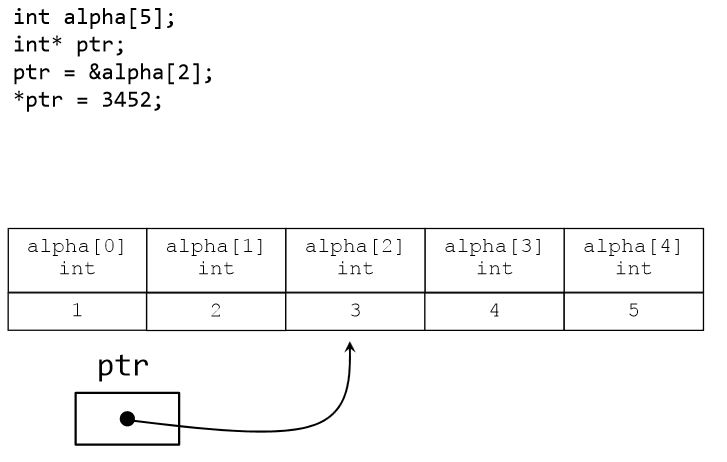
\includegraphics[width=0.6\textwidth]{pics/ptrAndVec.jpg}
    \end{minipage}
      \subsubsection{Vektor und Pointerarithmetik}
       \lstinputlisting[language=C,tabsize=2]{code/pointerarithm.c}
    
  \subsection{Zeichenketten}
   \lstinputlisting[language=C,tabsize=2]{code/strings.c}
  \subsection{Pointer und Referenzen als R"uckgabewert und Parameter"ubergabe}
  Bei Variablen"ubergabe (call by value) werden Kopien "ubergeben, welche nicht ver"andert werden k"onnen.\\
  Bei Referenz"ubergabe (call by reference) kann die Subroutine die Werte bleibend ver"andern.
  \begin{minipage}[t]{7 cm}
   \lstinputlisting[language=C,tabsize=2]{code/swap.c} 
   \end{minipage}
    \begin{minipage}[t]{10.5 cm}
      \lstinputlisting[language=C,tabsize=2]{code/swap2.c} 
      \end{minipage}
    
  \subsection{Zugriff auf Class und Struct Elemente}
  \lstinputlisting[language=C,tabsize=2]{code/classelem.c} 
